\section{Introduction}

Collecting large amounts of acoustic data from wild bird populations has
traditionally been very difficult. Due to technical limitations, studies have
often been constrained to tens of individuals and tens, or at best hundreds of
vocalisations. But this has changed rapidly within the last decade: compact and
economic autonomous recording units, such as the AudioMoth \parencite{hill2019}, now
make it possible to collect orders of magnitude more data from many more
individuals at once---and to do so much more cheaply. As a direct consequence,
many of the computational tools traditionally employed with bioacoustic data
have quickly become obsolete: they require manual curation, segmentation, and
labelling of data, which are extremely time-consuming and prone to errors.

To illustrate this point, as part of our research on a wild population of great
tits (\textit{Parus major}), we record around 50,000 songs every year, which
translates to well over half a million discrete acoustic units. Any analysis
that required finding, labelling, and characterising them, if done manually---as
is still often the case in wild bird vocalisation research \parencite{beecher2020a,
demko2018, mclean2020, pipek2018, youngblood2022}---would take a very long time to
complete. This bottleneck, in turn, severely limits researchers' ability to ask
questions that require large datasets to answer---such as those about social
learning, vocal development, large-scale cultural diversity, and the syntactic
organisation of animal vocalisations \parencite{aplin2019, kollmorgen2020,
lachlan2018, sainburg2019}.

In addition to concerns over the scalability of existing data analysis
pipelines, there is now a demand for tools that are freely accessible and
promote transparent, reproducible research. Existing proprietary software, such
as the widely used Raven Pro \cite[up to \$800,][]{raven2019} and Avisoft-SASLab
Pro \parencite[up to \$2,835,][]{specht2002} are difficult to reconcile with
contemporary data science practices that rely on open-source programming
languages such as R \parencite{rcoreteam2021} and Python \parencite{vanrossum1995}.
There exist some excellent open-source options, such as Luscinia
\parencite{lachlan2016a}, Sound Analysis Pro \parencite{tchernichovski2000} and the more
recent Koe \parencite{fukuzawa2020}. However, these were generally not designed to
cope with large volumes of data, and their reliance on point-and-click graphical
user interfaces limits their flexibility and hinders reproducibility.

%%%%% FIG 1
\begin{figure*}[t!]
    \centering
    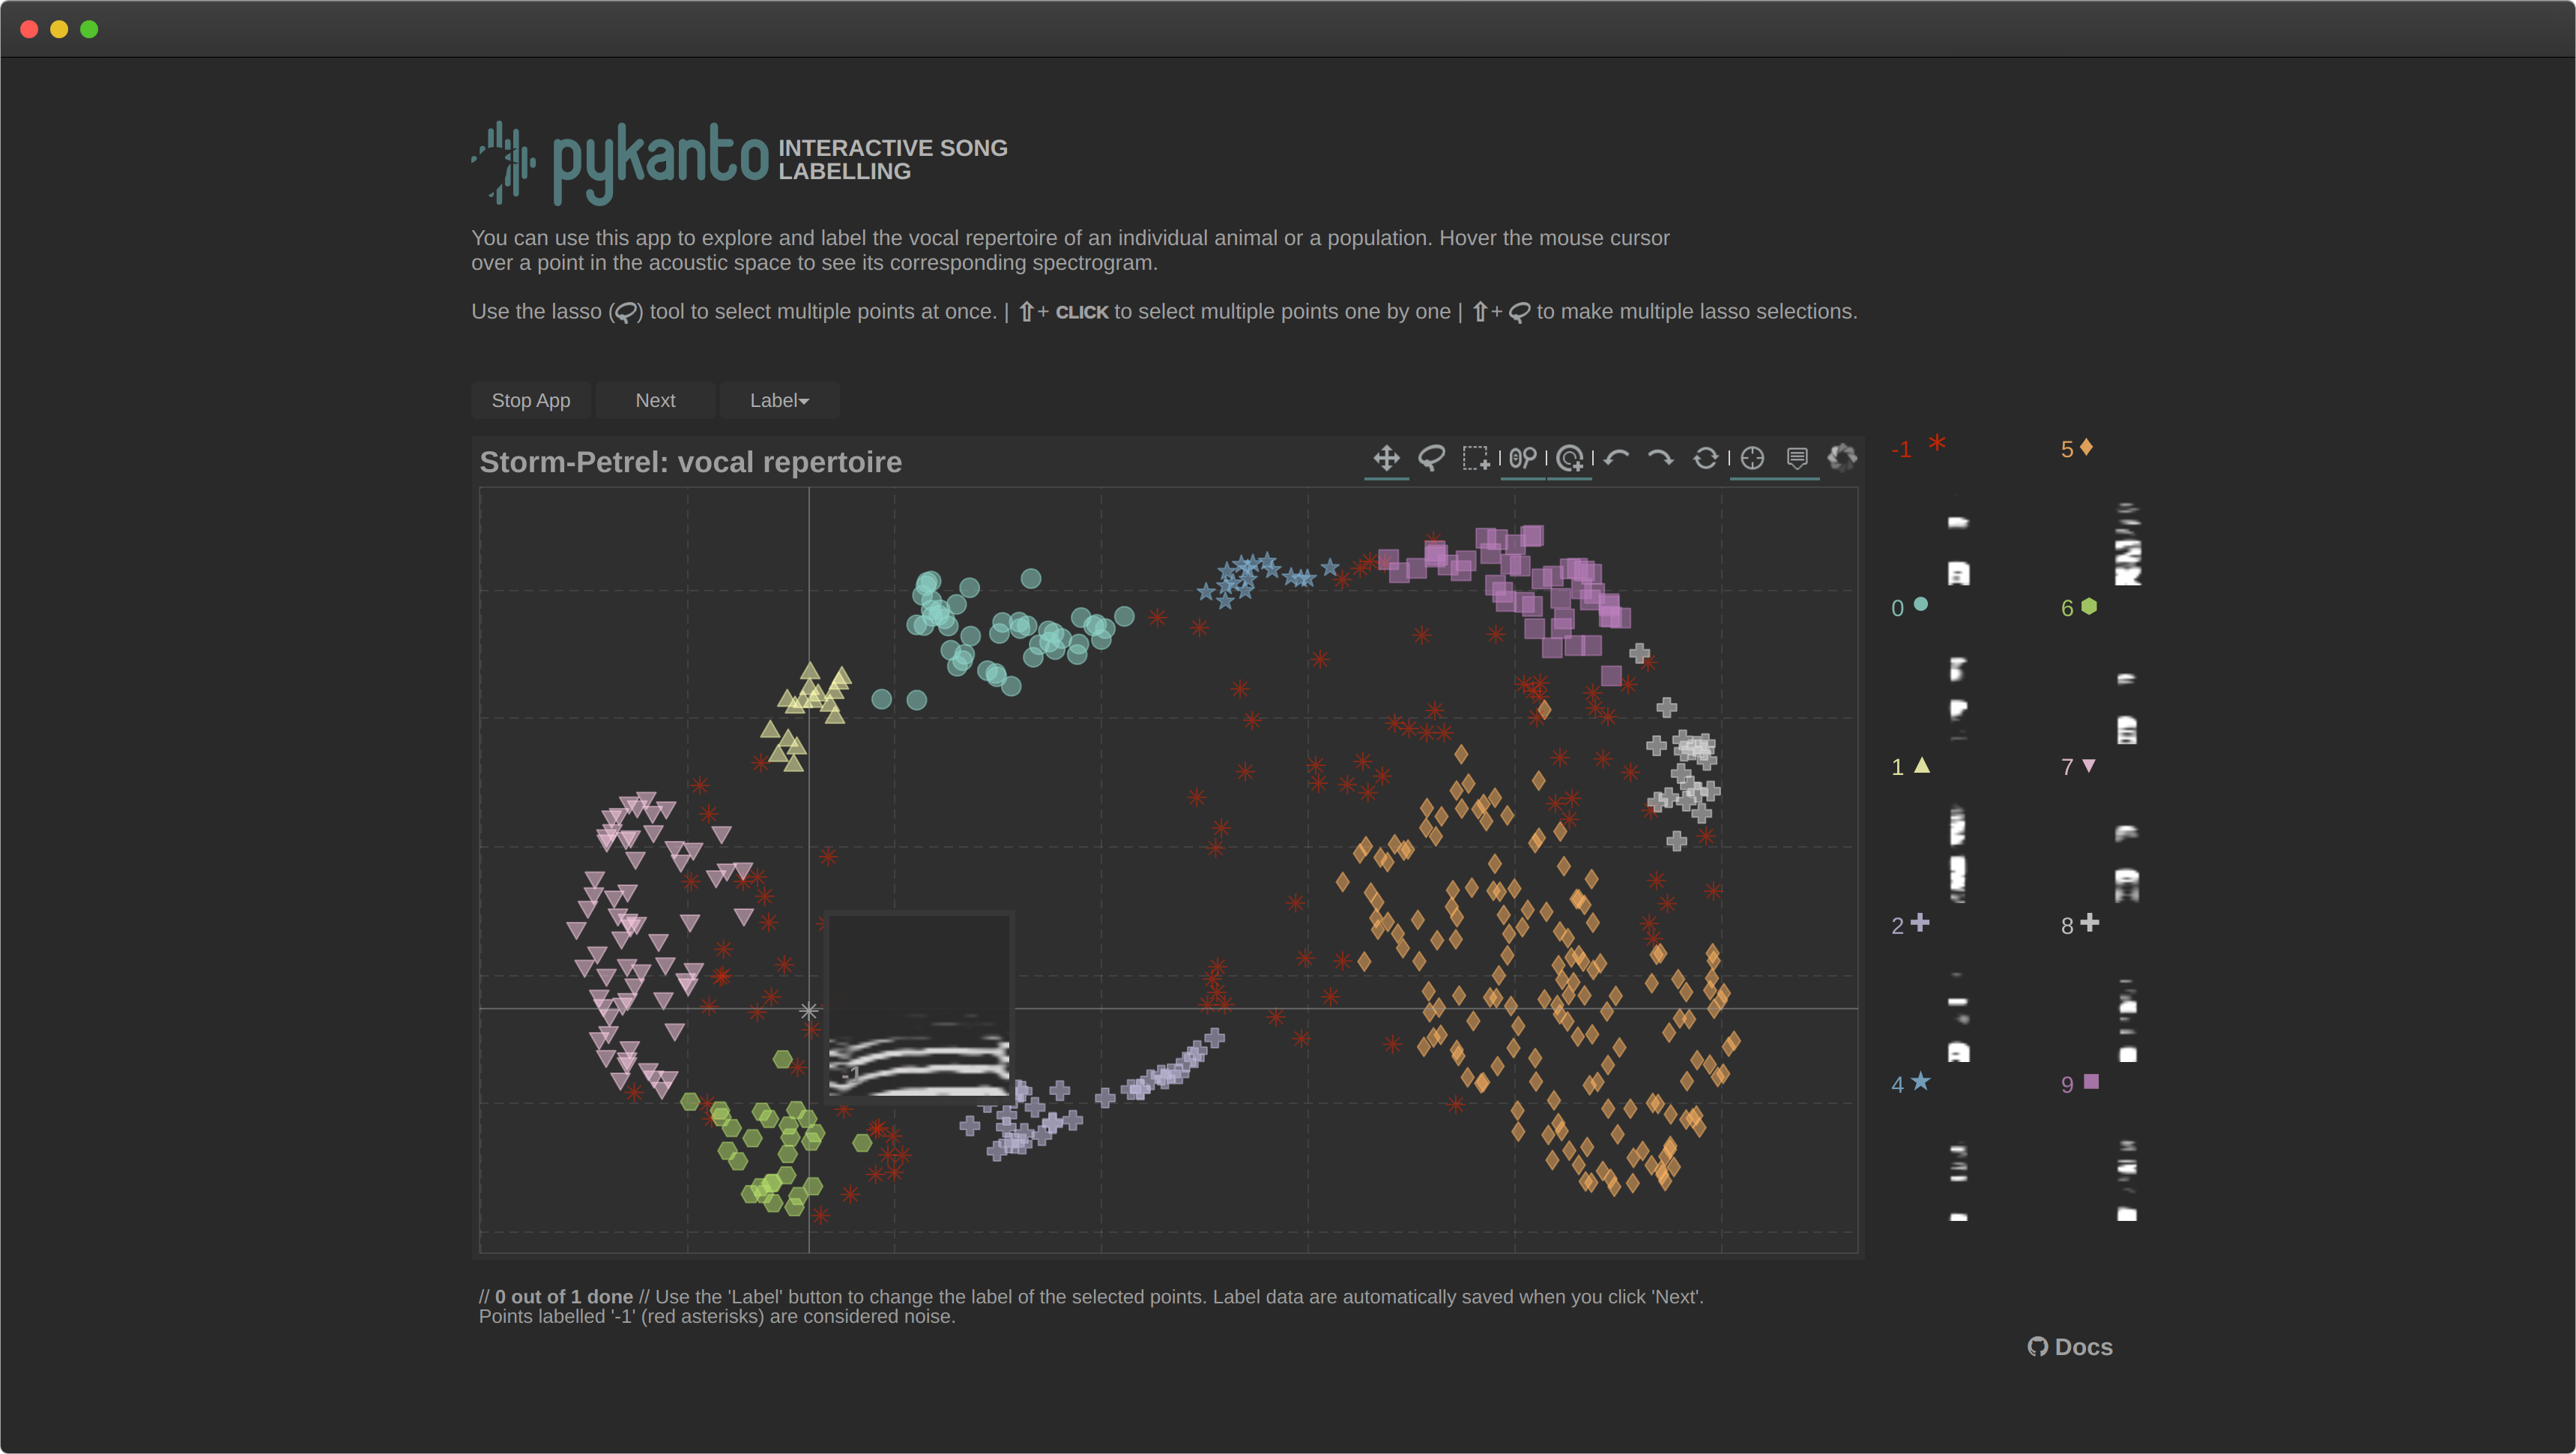
\includegraphics[width=\linewidth]{figures/chapter_2/fig1.png}
    \mycaption{Interactive web app to review and correct cluster assignment}{Interface of the interactive web app in pykanto. This app can be used to explore datasets as well as to review and correct automatically assigned class labels in bulk.}
    \label{fig:app}
\end{figure*}
%%%%%

As a response to the need for scalable and open-source tools for vocalisation
data analysis and related issues, the field of bioacoustics has recently started
to experiment with a new suite of methods based on deep-learning artificial
neural network architectures, the same that excel at, for example, computer
vision and speech recognition tasks \parencite{stowell2021}. Segmentation and
annotation pipelines based on deep neural networks have already been shown to
work well in laboratory settings, where three conditions hold: i) acoustic data
have a high signal-to-noise ratio, ii) there are orders of magnitude more
examples per vocalisation type than there are vocalisation types, and iii)
vocalisations are produced by relatively few individuals (fewer than ten to a
few tens) that do so in a stereotyped manner \parencite{coffey2019, cohen2022,
steinfath2021}. Unfortunately, none of these conditions tend to be the case in
field studies, and this creates a barrier to the adoption of new methods by
researchers working with natural populations.

This is the context in which I present \texttt{pykanto} (pronounced \textipa{pI·'kænt@U}). This software library was born of three needs, which can be summarised as follows.

\paragraph{First,} it needed to provide the infrastructure necessary to catalogue,
explore and label large acoustic datasets collected in often suboptimal field
conditions.

\paragraph{Second,} it had to serve as a flexible starting point that would allow researchers to perform both traditional analyses (such as extracting hand-picked
features from the vocalisations) and to use machine learning algorithms to learn
low-dimensional representations of the data \parencite{goffinet2021, kollmorgen2020,
morfi2021, sainburg2020}, train classifiers, or detect vocalisations in unseen
recordings \parencite{cohen2022, kahl2021, stowell2014}.

\paragraph{Third,} I wanted to build a tool that was free, open source, followed
sustainable software practises, and geared towards computational
reproducibility and transparency.

%%%%% FIG 2
\begin{figure*}
    \centering
    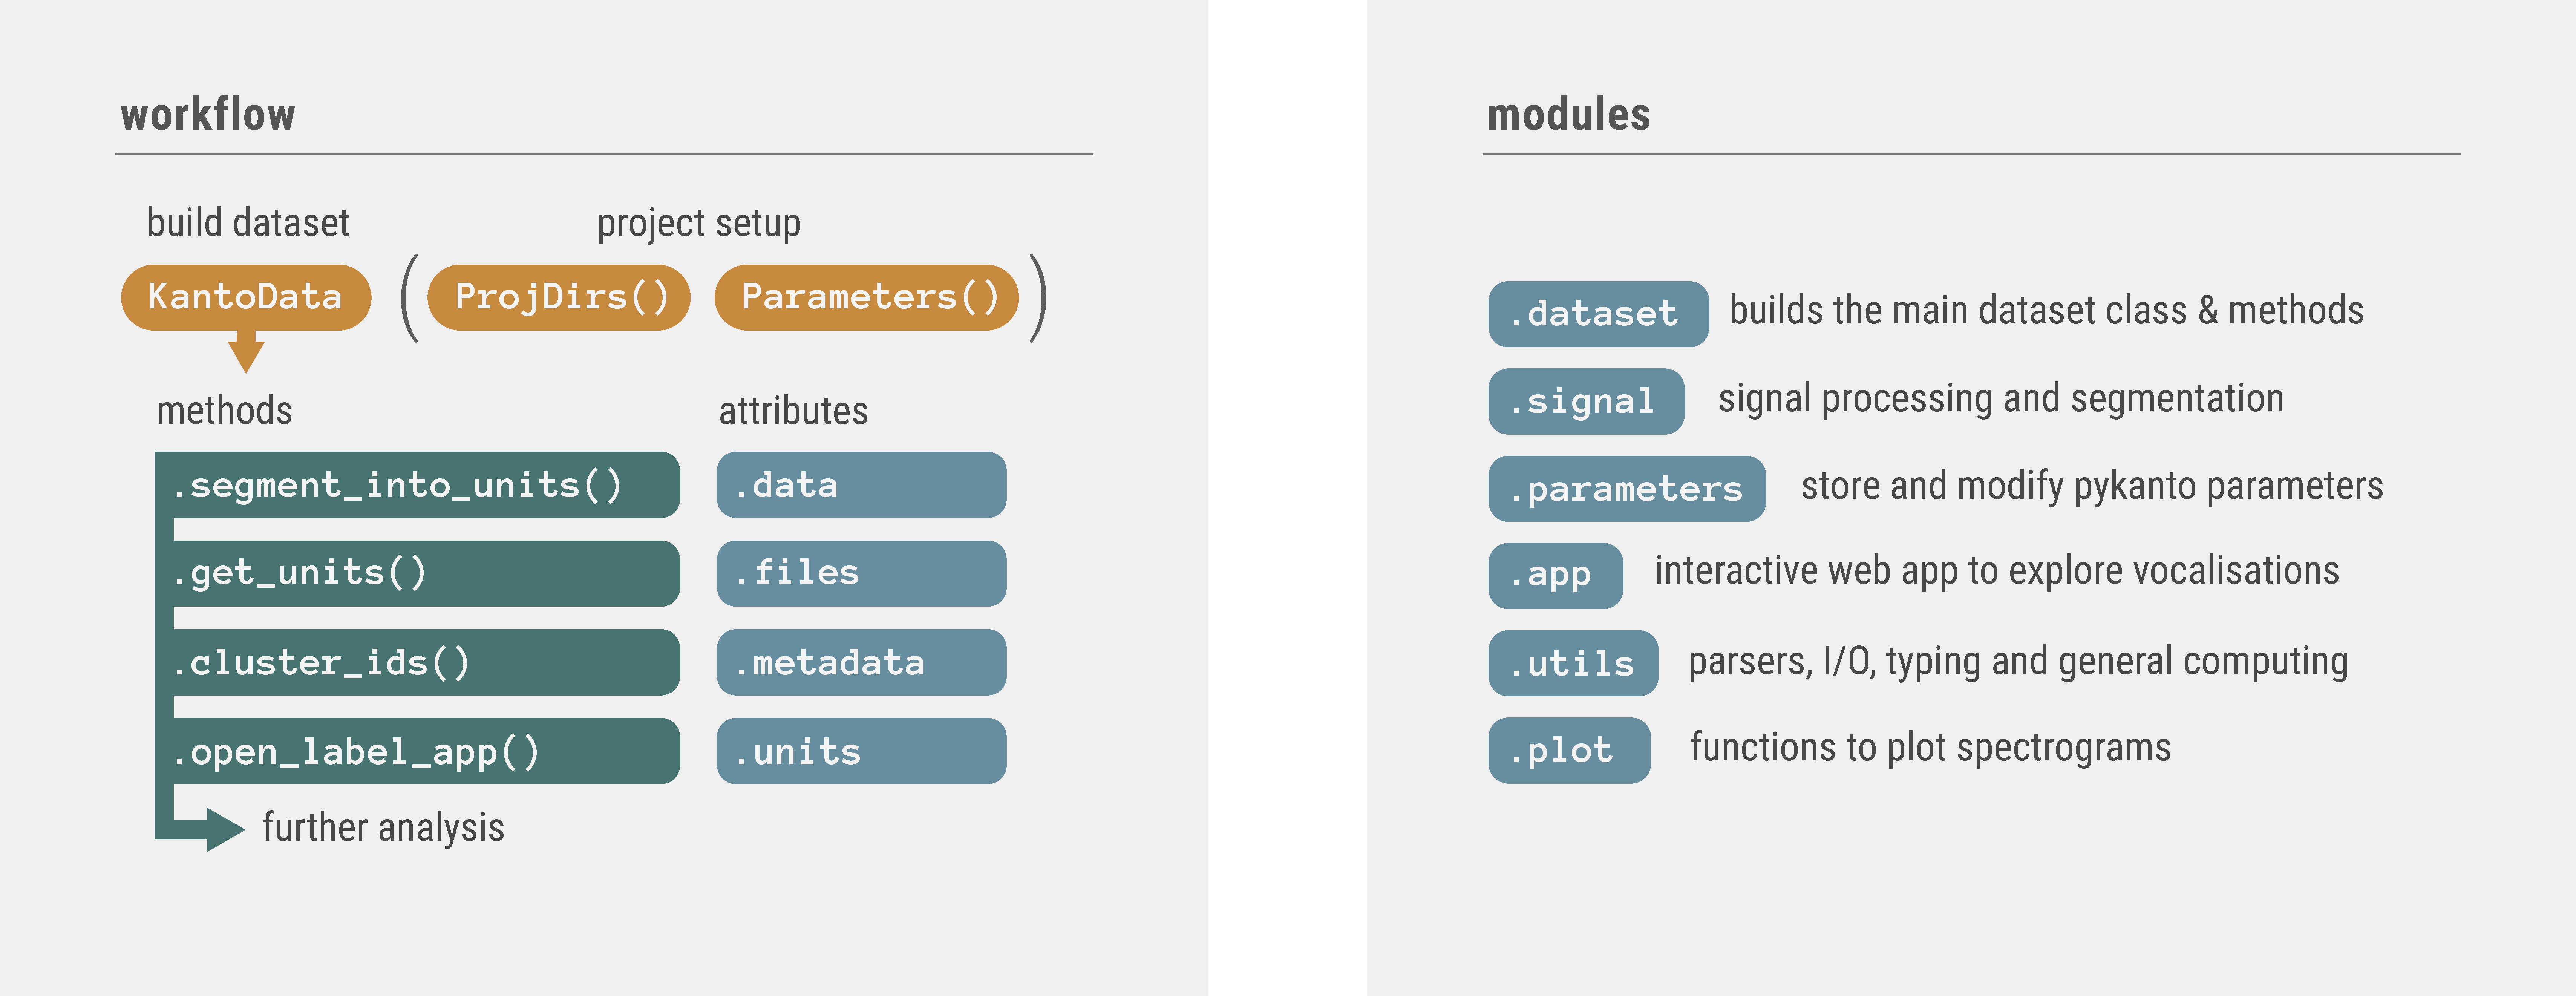
\includegraphics[width=0.6\textwidth]{figures/chapter_2/fig2.pdf}
    \mycaption{General structure of the library: main class and modules}{\texttt{pykanto} is written around a central dataset class, \texttt{KantoData}, which provides methods to segment, visualise and label vocalisations. The library contains six modules with functions and classes to carry out common tasks in animal vocalisation analysis.}
    \label{fig:structure}
\end{figure*}
%%%%%

\section{pykanto: Implementation}

\texttt{pykanto} is a software library designed to streamline the process of
analysing animal vocalisations. It is programmed in Python and offers various
modules to assist users in their work (see \autoref{fig:structure}). The central module is
\texttt{pykanto.dataset}, which serves as a database for vocalizations and
includes methods to visualise, segment, and label them. The \texttt{pykanto.signal} module provides tools for
signal processing and creating spectrograms, while \texttt{pykanto.parameters}
contains classes and functions for managing parameters. The web application
\texttt{pykanto.app} allows users to explore and label large numbers of
vocalizations (\autoref{fig:app}) and \texttt{pykanto.plot} provides functions for
plotting spectrograms. Finally, \texttt{pykanto.utils} includes parsers, I/O
tools, custom typing, and general computing functions. The documentation for
\texttt{pykanto} is available at
\href{https://nilomr.github.io/pykanto}{\nolinkurl{nilomr.github.io/pykanto}}.

\subsection{Dependencies}

\texttt{pykanto} was written in Python 3.8 and tested in Python 3.8, 3.9 and
3.10. Its interactive web application also relies on JavaScript, HTML, and CSS.
External dependencies are automatically downloaded during package installation
(see the
\href{https://github.com/nilomr/pykanto/blob/main/pyproject.toml}{\texttt{pyproject.toml}}
file for a full list of dependencies).

\subsection{API and documentation}

\texttt{pykanto} is a well-documented code library, making it easier to use and
contribute to its development. The methods and functions in \texttt{pykanto} have clear
and concise documentation, including type annotations and descriptions of their
intended use. Its API (Application Programming Interface) reference, along with
tutorials and practical examples, can be found in the online documentation
at \href{https://nilomr.github.io/pykanto}{\nolinkurl{nilomr.github.io/pykanto}}.

\subsection{Reproducibility and open research}

\texttt{pykanto} encourages the user to create reproducible data science
projects. For example, one of its modules is dedicated to creating consistent
project structures, inspired by popular utilities such as
\href{https://github.com/cookiecutter/cookiecutter}{cookiecutter}. Using the
library requires writing simple scripts in Python, which allows every step of
the research, from data ingestion to eventual model training and reporting, to be
explicitly reproduced. The documentation includes a complete user guide with
examples of best practices.

The input and output files use open data formats, and all code is available
under the \href{https://choosealicense.com/licenses/mit/}{MIT licence} (a simple
and very permissive licence). Where applicable, we have followed the guidelines
and recommendations of the Software Sustainability Institute, a UK-based
facility dedicated to research software sustainability
(\href{https://www.software.ac.uk/}{software.ac.uk}).



Many of the processes that \texttt{pykanto} carries out are computationally
intensive, such as calculating spectrograms, performing operations on large
arrays, and running dimensionality reduction and clustering algorithms.
High-level, interpreted languages---like R or Python---are notoriously slow: where
possible, we have optimised performance by both a) translating functions to
optimized machine code at runtime using Numba \parencite{lam2015} and b)
parallelising tasks using Ray, a state-of-the-art platform for distributed
computing \parencite{moritz2018}. As an example, the \texttt{segment\_into\_units()}
function can find and segment 20.000 discrete acoustic units in approximately
16s on a desktop, 8-core machine; a dataset with over half a million (556.472)
units takes ~132s on a standard 48-core compute node. If \texttt{pykanto} detects a
suitable GPU unit and the optional dependencies are installed, algorithms such
as UMAP \parencite{mcinnes2018} switch to their GPU implementation, which provides a
15-100x speedup \parencite{nolet2021, raschka2020}. The library has a module
dedicated to making it easy for users to run their scripts in a high-performance
computing context (for example, a university compute cluster), and its
documentation includes examples of configuration and submission scripts.

\subsection{Limitations}

This final section discusses some of the main limitations of \texttt{pykanto}. Although it
will hopefully offer a flexible solution for researchers, it is also limited in
important ways.

\paragraph{Limitation 1} Vocalisation unit segmentation via the very simple amplitude
thresholding algorithm will not work well with species whose vocalisations vary
greatly in amplitude, or with very noisy datasets. In those cases, and depending
on data volume,  segmentation might better be performed either manually or in a
semi-automated way. For example, one could use \textit{chipper}
\parencite{searfoss2020a} or train a neural network like TweetyNet,
\parencite{cohen2022} on a manually annotated subset of the data.

\paragraph{Limitation 2} \texttt{pykanto} has been tested on species that produce
vocalisations made up of a small or moderate number of different but distinct
elements (variously referred to as notes or syllables). It will be useful for
researchers working with any species, but the automatic part of the clustering
process will work increasingly poorly with those that have a large number of
very variable elements. This is true of any clustering method: they will fail or
produce spurious results if variation in the data is continuous.

\paragraph{Limitation 3} The library does not include methods to train models intended to
find analysable vocalisations in long recordings of entire soundscapes. This is
a particularly challenging problem \parencite{priyadarshani2018} without a universal
solution. However, \texttt{pykanto} can be used to generate and organise the training
data required by these models \parencite{kahl2021, stowell2019, stowell2014}, and to
work with their output annotations.

\paragraph{Limitation 4} \texttt{pykanto} is intended as a flexible solution for managing
and preparing animal vocalisation data for further analysis. It provides tools
that can save researchers a great deal of time while making analysis pipelines
more reproducible. However, it does not implement any specific analysis or
feature extraction methods, since these will vary greatly by use case. This
means that researchers using the library as part of their work will need to
either have or develop familiarity with bioacoustic analysis and scripting in
Python.

\section{Using pykanto: can individual birds be identified from their songs?}

I now provide a worked example of how \texttt{pykanto} can be used to help answer real research questions about vocalisations---bird song in this case:

\subsection{Introduction}

Great tits are small, short-lived birds (average lifespan: 1.9 years) that sing
acoustically simple yet highly diverse songs. In Wytham Woods, Oxfordshire (UK),
a population of these birds has been the focus of a long-term study that is now
in its 75th year. For the past three years, I have recorded the song repertoires of
hundreds of individual males when they sing close to their nest before their
partner begins laying. With the help of these data, we are trying to answer
questions about song learning and cultural change in natural populations.

To do this we first need to know which individuals are present in the breeding
population for the first time, and which were already around in previous years.
However, individual survival over the winter months is low and detection by
traditional means---such as mist-netting or identification in the nest---is
imperfect. So we would first like to test whether individual birds can be
identified based on their songs alone, and then quantify how much variation in
song types occurs within and between years.

Our example dataset consists of 5293 songs from 12 males that were known (from
physical recaptures) to be present in the breeding population in two different
years, 2020 and 2021. Although this is a small subset of our data, it is large
enough that it would still take weeks to process and analyse using traditional
methods. We demonstrate the use of \texttt{pykanto} to a) organise, segment and label the
dataset, and b) prepare it so that we can train a deep neural network to
recognise the bird's song types. The entire process, which takes under an hour to complete,
can be computationally reproduced using its
\href{https://github.com/nilomr/pykanto-example}{dedicated
repository}. The repository includes
raw data, auxiliary scripts and detailed instructions. Below is a short
narrative description of the process.

\subsection{Data collection}
Most great tits in our population nest in nest boxes with known locations. Every year, fieldworkers record the identities of breeding males and females, clutch initiation and egg-hatching dates, clutch size, and fledgling success using standardized protocols. A significant number of birds in the population are fitted with a unique British Trust for Ornithology (BTO) metal leg ring as nestlings or adults. During the breeding season (March to June), great tit pairs are socially monogamous and protect territories around their nest boxes \parencite{hinde1952}.

We collected data during the breeding seasons of 2020 and 2021, from early April to late May, using a dense sampling design with multiple recorders placed in nest boxes throughout the study site. Fieldworkers checked every nest box in the study site at least once a week before and during egg laying, which can last from one to 14 days \parencite{Perrins1965}. Once a nest box was believed to be in use by a great tit, we placed an autonomous sound recorder in its vicinity, either in the same tree or in a suitable neighbouring tree. We left each recorder in the same location for at least three consecutive days before moving it to a different nest box. Throughout the recording period, we relocated 20 recorders every day.

We used 60 AudioMoth recorders \parencite{hill2019} in 2021 and 30 in 2020, which were housed in waterproof custom-built enclosures. Recording began about an hour before sunrise (from 05:36 to 04:00 UTC during the recording period) and consisted of seven 60-minute recordings with a sample rate of 48 kHz. Since the recording process was automated, there is a possibility that some of the songs recorded in the immediate vicinity of a given nest box do not belong to the focal bird. To reduce the risk of false positives, we discarded recordings with more than one vocalizing bird, unless one was distinctly louder than the others. We also discarded all songs with a maximum amplitude below $-16 dB$, calculated as $20\log_{10} \left (\frac{A}{A_{0}}\right )$, with $A = 5000$ and $A_{0} = 32767$ (the maximum value for 16-bit digital audio). This threshold was determined from the observation that, in cases where we had simultaneous recordings of close neighbours from the centres of their respective territories, an amplitude cutoff greater than 4000 always separated a focal bird from its neighbours. It should be noted that these values are not calibrated and are relative to the recording equipment and settings used, as well as other factors such as sound directionality and vegetation cover.

\subsection{Running the analysis}
\subsubsection{Installation}

\texttt{pykanto} can be used outside a virtual environment, but this is not encouraged.
Using clean environments for each project will allow you to avoid dependency issues. Once inside a new environment with Python 3.8 or above, you can
install \texttt{pykanto} by simply running \texttt{pip install pykanto}, then install the
package containing this example. See detailed installation and use instructions
in the \href{https://github.com/nilomr/pykanto-example}{\texttt{.README}}.

\subsubsection{Creating a new project and dataset}

Our first step will be to define a directory structure for our project and a
\texttt{ProjDirs} object to hold everything together. Then, we can test and set
adequate parameters for our dataset. These include things like low- and high-cut
filters, spectrogram settings, amplitude thresholding, and whether the analysis
will be carried out at the song or note level. The data folder in the project
already contains \texttt{.wav} audio files and their corresponding
\texttt{.json} with annotations, so we can create a \texttt{KantoData} instance:
this will be our database.

\subsubsection{Segmenting songs and using the interactive app}

Then, using the \texttt{.segment\_into\_units()} method, we find segment onsets,
offsets, unit and silence durations and add them to \texttt{KantoData.data}, the
main data frame in our database object. At this point, we could already carry
out most of the analyses common in the bird song literature, for example, by
extracting some simple acoustic parameters from the segmented data. Instead, we
want to preserve all the temporal and spectral information that is available in
the spectrograms to train a more accurate classifier.

The next step is to compute and store spectrograms for each unit under
examination, and then reduce their dimensionality and group them into clusters.
This can be achieved by using the \texttt{.get\_units()} and \texttt{.cluster\_ids()} methods, which
employ algorithms such as UMAP \parencite{mcinnes2018} and HDBSCAN
\parencite{mcinnes2017}. Afterwards, we can launch the interactive web app by
calling \texttt{.open\_label\_app()}. Using this app, we can review the automatic labels
for up to tens of thousands of vocalisations at once, splitting or combining
clusters as needed. Once completed, we will have a fully annotated dataset, which
can be divided into training and testing sets and exported as labelled
spectrograms using \texttt{pykanto}. 



%%%%% FIG 3
\begin{figure*}
    \centering
    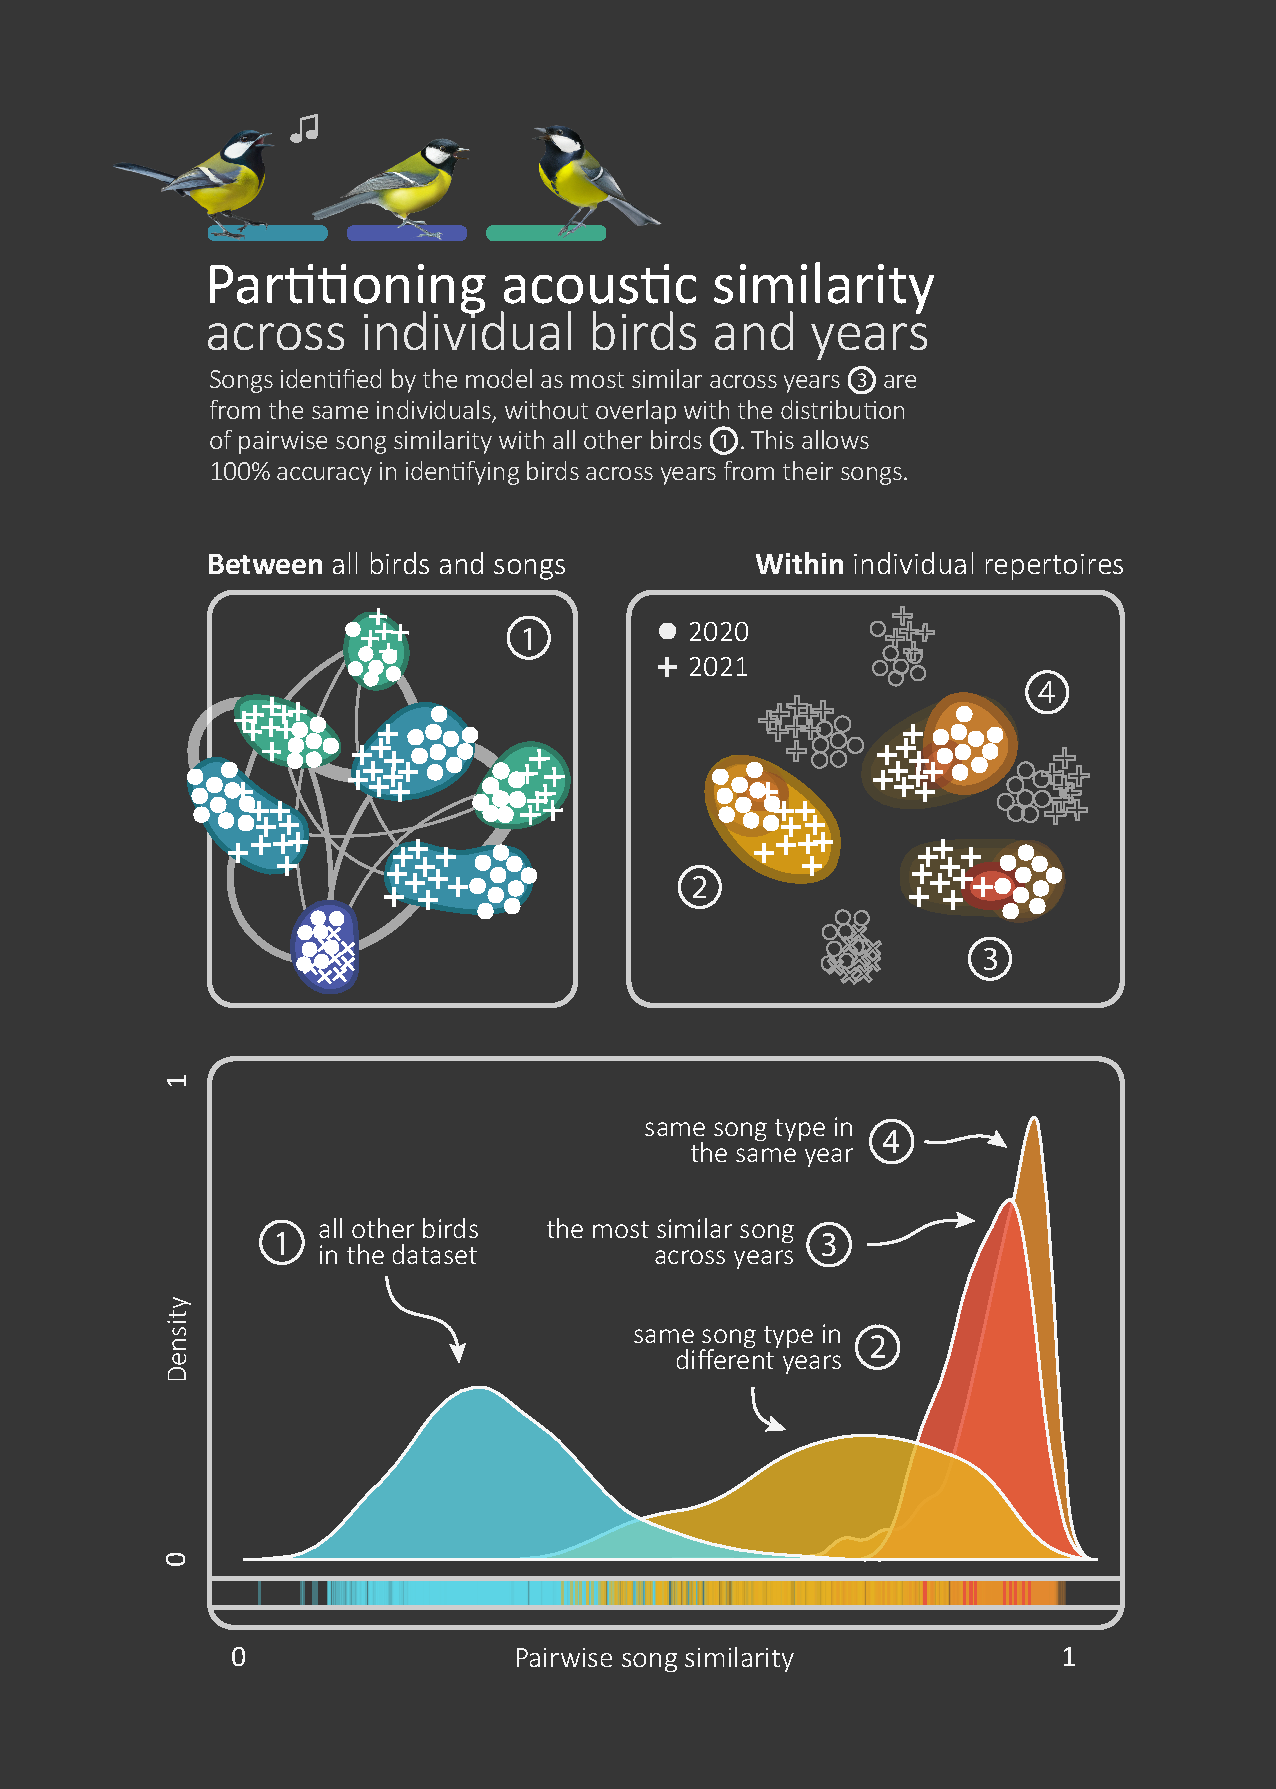
\includegraphics[width=\linewidth]{figures/chapter_2/fig3.pdf}
    \mycaption{Partitioning acoustic similarity between and within birds}{(From left to right and top to bottom.) First, we calculate the pairwise similarity between the songs of all birds, which provides a baseline distribution of similarity in the population (1). Then, we compare songs from the same bird in different years (2), find the pair of songs that are most similar across years (3), and compare songs within the same year (4). The probability density estimates in the bottom panel show how pairwise similarities in (3) allow us to re-identify birds across as they do not overlap with any other birds (1).}
    \label{c2_fig:results}
\end{figure*}
%%%%%

\subsubsection{Training a convolutional neural network classifier}
Our goal is to generate compressed representations of songs that can facilitate comparisons and identification of those sung by the same individual, even in the presence of variations in performance and noise. To do this, we can train a model to distinguish between different song types, which are categorically distinct within individual song repertoires, without providing the model with information about who sang them. 

In this example, we use weights from a pre-trained ResNet50 backbone \parencite{he2015} and gradually unfreeze the earlier layers of the network during training. By doing so, we can fine-tune the network to attain better performance in our task, while still benefiting from the weights learned on a much larger dataset \parencite{zhuang2021}. 

The distribution of song sample sizes per individual approximately follows a
power law, so there is a very large amount of data for a few birds and very
little for most. This imbalance of data is problematic for learning algorithms, as they may develop a bias toward larger classes and perform poorly on rarer ones. There are different ways to deal with this \parencite[see, e.g.,][]{krawczyk2016, thabtah2020}; however, to keep things simple, here we will just undersample majority classes so that all birds have the smallest common sample size for each song type.

Background noise can also bias our analysis. Each bird's acoustic environment is unique, and the network may learn to distinguish between songs based on this noise rather than the signal of interest. To address this issue, we remove most background noise by thresholding the spectrograms, taking advantage of the difference in amplitude between the focal bird singing near the recording and its acoustic background. Additionally, we apply a series of data augmentation techniques during the training process to prevent over-fitting and ensure that the algorithm does not memorise irrelevant or highly variable elements. These techniques include semi-random cropping in the time domain, blurring and sharpening, random erasing of parts of the spectrogram, and contrast and brightness changes. After training the model, we can verify that background noise is not causing bias by checking whether songs recorded in the same location are classified as more similar than expected by chance. In addition, we can create class activation maps to identify the regions of the spectrograms used by the model to generate predictions.

Once the model is trained, we can assess its ability to classify unseen songs drawn from the held-out dataset, which can reach an accuracy of around 92\%. As described below, most of the remaining 8\% can be attributed to confusion between the same song types sung by the same birds in different years. 

Finally, we can use the model to extract a compressed representation of each song in the entire dataset. This is achieved by passing each song through the trained network and obtaining the output from the last hidden layer. This output consists of a feature vector that captures the most relevant information to distinguish between different types of songs; these feature vectors can then be used to determine whether two songs are very similar. In our case, we do this by taking the inverse of the cosine distance between each pair to build a similarity matrix.

The repository that supports this paper contains a streamlined way of doing this using PyTorch (\citeyear{pytorch2019}) and PyTorch Lightning (\citeyear{pytorchlightning2019}) that can be easily adapted for use with other datasets.


\subsection{Results \& Discussion}

After calculating the similarity scores between all pairs of songs, we grouped them according to song type, the bird that sang them, and the year they were sung. For each bird in the first year, we identified the individual who sang the song with the highest similarity to any within its repertoire during the following year. We found that we were able to successfully identify the correct bird in all cases, even though the baseline probability was only 2.27\% (1 out of 44 song types). This suggests that we would have been able to re-identify the individuals even if they had not been observed or captured again.

As shown in \autoref{c2_fig:results}, the highest similarity values correspond to
comparisons of the same song types within years and birds. The similarity
between the same song types sung by the same bird across different years is
consistently higher than that between different birds, even when some song types were shared by individuals: this means that individual vocal signatures are
at least partly maintained across their lifespan.

The conclusions drawn from this analysis are limited by the small size of the
dataset: including more birds would likely lead to noisier results, as it increases the chances of finding a second bird with even more similar songs. Nonetheless, in
combination with other information (such as spatial location), they might allow
high-confidence identification of individuals between years without physical
capture.

This example illustrates how \texttt{pykanto} can be used to help address a
specific research question. The model-based feature vectors used to describe each song
can be imported back into the \texttt{KantoData} database as a new column, enabling a
wide range of research possibilities while maintaining a clear project
structure.

\section{Data availability}

We distribute \texttt{pykanto} with three sample datasets that are used to run unit tests
and as examples in the documentation \parencite{nilo_pykanto_2023}.

\paragraph{Great tit songs} 20 songs recorded from male birds during the dawn chorus in a
population in Oxford, UK. Recorded by the author and accessible at \href{https://github.com/nilomr/pykanto/tree/main/pykanto/data/segmented/great_tit}{pykanto/data/great\_tit}.

\paragraph{European storm-petrel purr songs} Two males singing from burrows in the Shetland
and Faroe islands. Source: \href{https://xeno-canto.org/46092}{XC46092} (©
Dougie Preston), \href{https://xeno-canto.org/663885}{XC663885} (© Simon S.
Christiansen). Under
\href{https://creativecommons.org/licenses/by-nc-nd/2.5/}{CC BY-NC-ND 2.5
licence}.

\paragraph{Bengalese finch songs} Recordings from 2 isolated Bengalese finches. Originally
published in Tachibana, Koumura and Okanoya \parencite{tachibana2015}, data can be
accessed at \href{https://osf.io/r6paq/}{OSF}.\par

They can be found under \texttt{pykanto/data} when you install the package, as well as in the \href{https://github.com/nilomr/pykanto}{GitHub repository}.

\paragraph{}Additionally, the worked example in this article uses 5293 songs from male great tit songs recorded by the author between 2020 and 2021 in Wytham Woods, Oxfordshire, UK. They are available from \href{https://github.com/nilomr/pykanto-example/tree/main/data/segmented/pykanto-example}{pykanto-example/data} on GitHub, along with detailed metadata \parencite{nilo_pykanto_example_2023}.

\section{Code availability}

The latest version of \texttt{pykanto} is available from PyPI (\texttt{pip install
pykanto}) and its source repository (\href{https://github.com/nilomr/pykanto}{github.com/pykanto}). See the repository for detailed installation instructions.

\texttt{pykanto} and the example in this article rely on the following open-source scientific
libraries or tools: numpy \parencite{numpy2020}, scipy \parencite{scipy2020}, pandas
\parencite{pandas2023}, numba \parencite{lam2015}, pytorch \parencite{pytorch2019},
torchvision \parencite{torchvision2016}, pytorch lightning
\parencite{pytorchlightning2019}, tqdm \parencite{tqdm2019}, ray \parencite{moritz2018},
soundfile \parencite{bechtold2022}, umap \parencite{mcinnes2018},  joblib
\parencite{joblib2020}, hdbscan \parencite{mcinnes2017}, seaborn \parencite{Waskom2021},
scikit-image \parencite{scikitimage2014}, librosa \parencite{mcfee2015}, bokeh
\parencite{bokeh2018}, ujson \parencite{ujason2023}, psutil \parencite{psutil2023}, attrs
\parencite{schlawack2019}.

\section{Acknowledgements}

I thank Ben Sheldon and the Sheldon lab for their support and
patience. Ben Sheldon, Carys Jones and Andrea Estandia provided useful comments on a draft of this
manuscript. Carys Jones and Antoine Vansse tried early versions of the
interactive app in \texttt{pykanto} and provided valuable feedback.

Some of the methods in \texttt{pykanto} are directly inspired by or adapted
from \cite{sainburg2020}. I have indicated where
this is the case in the relevant method's docstring. The dereverberation
function is based on code by Robert Lachlan that is part of Luscinia
\parencite{lachlan2016a}, a software for bioacoustic archiving, measurement and
analysis. Please consider citing these two publications if you use
\texttt{pykanto} on your own projects.

I have learnt a great deal about packaging and developing in Python by browsing
the structure of existing open source projects, for example some by David
Nicholson (\href{https://github.com/NickleDave/NickleDave}{@NickleDave}). I only
became aware of \href{https://github.com/vocalpy}{VocalPy}, a project that aims
to "develop an ecosystem of interoperable packages" for
"computational vocal communication and learning research" when I had
already written most of \texttt{pykanto}, but eventually, I would like to make it
compatible with it: standardisation is direly needed in the field and I don't
want to contribute to the chaos.

This work was supported by a Clarendon-Mary Frances Wagley Graduate Scholarship
and an EGI scholarship to Nilo Merino Recalde, and made use of the University of Oxford Advanced
Research Computing facility \parencite{richards2015}.

\section{Conflict of interest}

The author declares no conflict of interest.

\section{Author contributions}

Nilo Merino Recalde wrote the software library and its documentation, collected the data,
conducted the analyses, and wrote the manuscript.

\renewcommand{\cleardoublepage}{}
\renewcommand{\clearpage}{}
\printbibliography
